\documentclass[thesis.tex]{subfiles}

\begin{document}

\chapter{KdV5}

\section{Periodic 2-pulse}

In this section, we will consider the simplest case, which is the periodic 2-pulse. Let $Q_2(x)$ be a periodic 2-pulse constructed as in Theorem \ref{perexist} with scaling parameter $r$, baseline length parameters $\{b_0^0, b_1^0 \}$ with $b_j^0 = \exp\left(-\frac{m_j \pi}{\rho}\right)$, and phase parameter $\theta$. Without loss of generality, $m_0 \in \{0, 1\}$. Let $b_0(r)$ and $b_1(r)$ be the associated length parameters, and let $X_0$ and $X_1$ be the actual pulse distances, whose dependence on these parameters is given in Theorem \ref{perexist}. Finally, let $X = X_0 + X_1$.  

By Theorem \ref{blockmatrixtheorem} [Theorem 5.4, the block matrix theorem], the eigenvalues for the linearization about $Q_2(x)$ can be found by finding the zeros of the determinant of a block matrix. To leading order, this is block diagonal. We expect to find the interaction eigenvalues when $A - \lambda^2 M I$ is singular and the essential spectrum eigenvalues when $K(\lambda)$ is singular. Thus we anticipate the following eigenvalue pattern.
\begin{itemize}
\item There will be a pair of nonzero interaction eigenvalues at $\lambda = \pm \sqrt{-2a(r)/M}$, where 
\[
a(r) = a_0(r) + a_1(r) = \langle \Psi(X_0), Q'(-X_0) \rangle + \langle \Psi(X_1), Q'(-X_1) \rangle = \mathcal{O}(r)
\]
\item There will be essential spectrum eigenvalues at
\[
\lambda = \pm c \frac{k \pi i}{X}
\]
for integer $k$, where $X = \mathcal{O}(|\log r|)$.
\end{itemize}

We are interested in two parameter regimes. First, we will consider the case where $r$ is sufficiently small so the interaction eigenvalues are smaller in magnitude than the essential spectrum eigenvalues. Next, we will consider the case when a purely imaginary interaction eigenvalue is close to the first nonzero essential spectrum eigenvalue, which case we will have an instability bubble.

\subsection{Case 1: essential spectrum is out of the way}\label{section:2pernobubble}

In this section, we consider the case where the essential spectrum is ``out of the way'' of any interaction eigenvalues. Since the interaction eigenvalues scale like $r^{1/2}$ and the essential spectrum eigenvalues scale like $1/|\log r|$, we can always choose $r$ sufficiently small so that this is the case. We therefore expect that the eigenvalues will come in one of the two patterns shown in \cref{fig:2ppatterns}.

\begin{figure}[H]
\begin{center}
\begin{tabular}{cc}
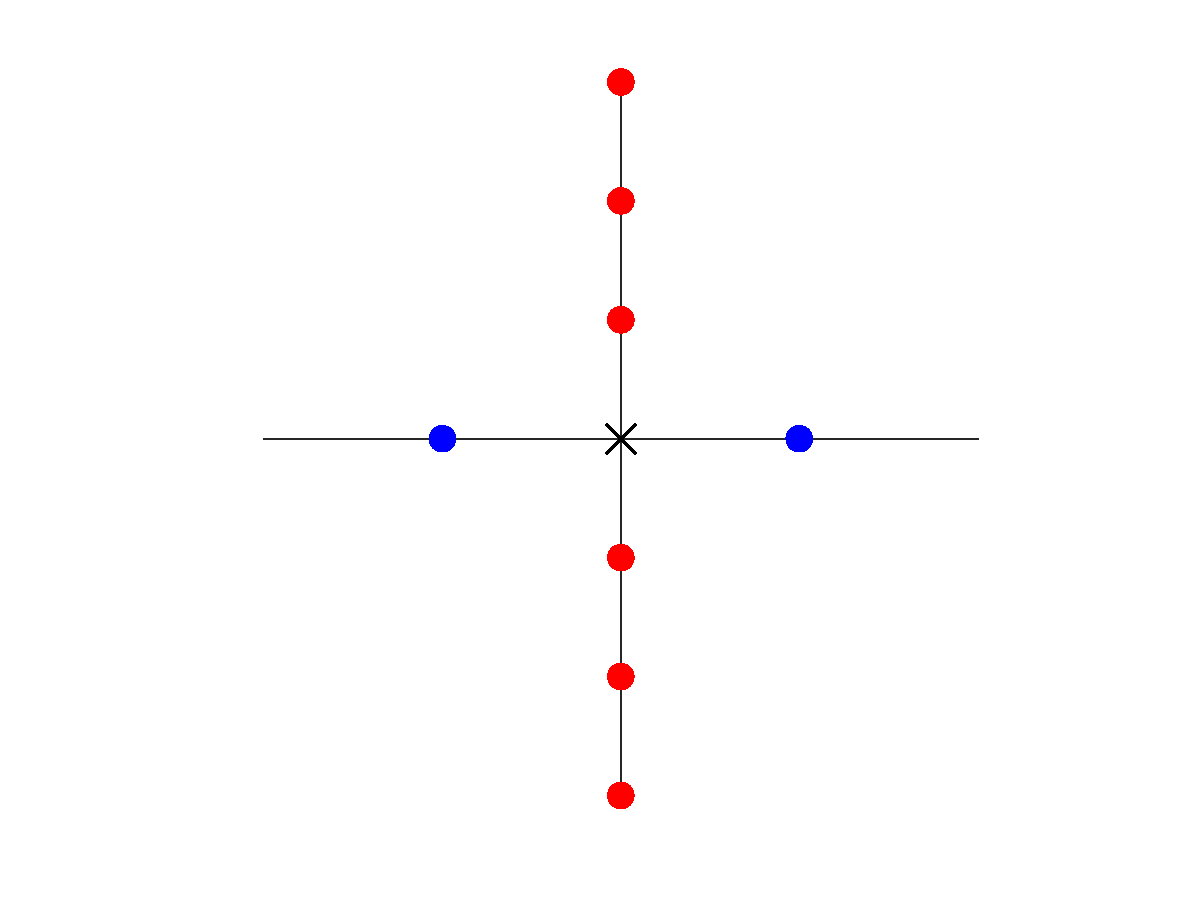
\includegraphics[width=5cm]{images/kdv5/2punstableeigpattern.eps} &
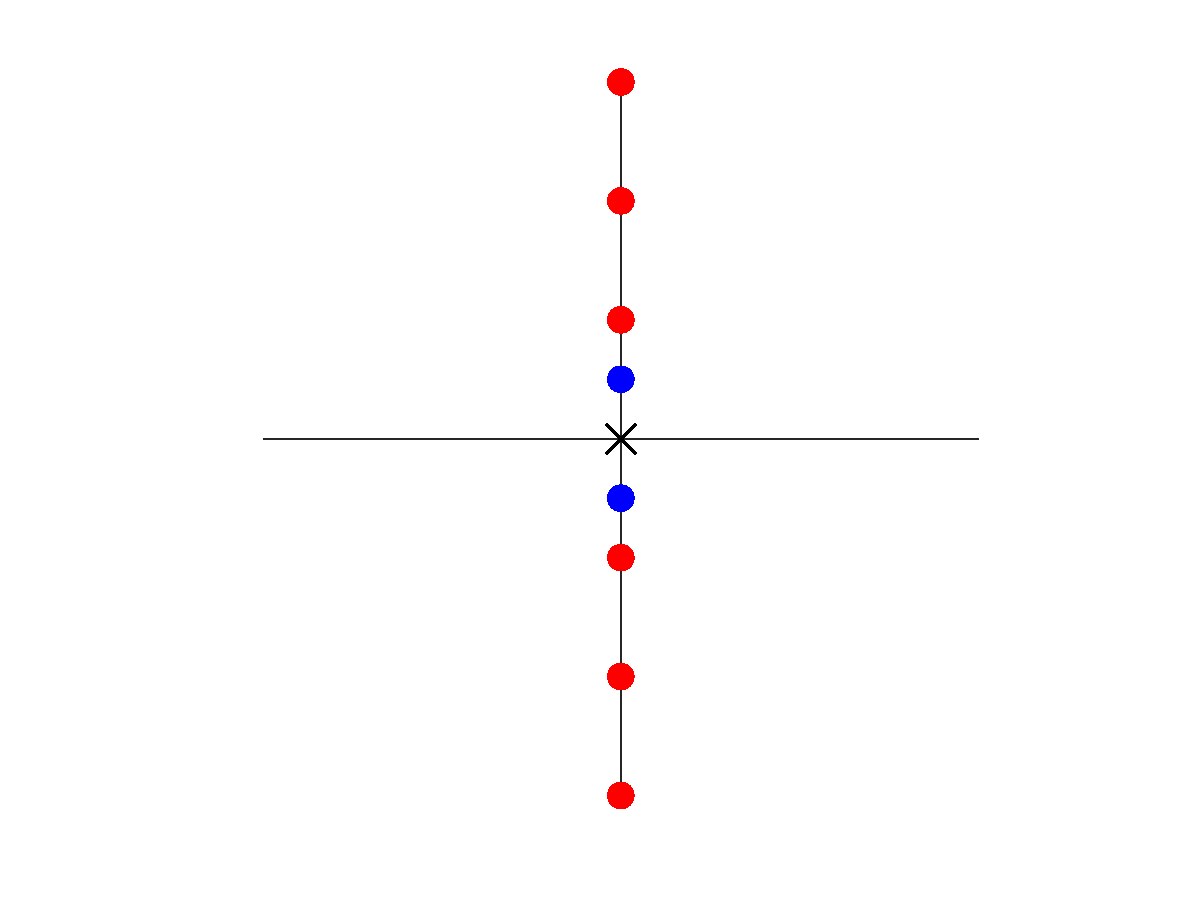
\includegraphics[width=5cm]{images/kdv5/2pstableeigpattern.eps} 
\end{tabular}
\caption{Eigenvalue patterns for periodic 2-pulse with essential spectrum out of the way. Blue dots are interaction eigenvalues, red dots are essential spectrum eigenvalues, and black X at the origin represents the three kernel eigenvalues. Left panel shows a pair of real interaction eigenvalues, and right panel shows a pair of purely imaginary interaction eigenvalues. }
\label{fig:2ppatterns}
\end{center}
\end{figure}

In the next theorem we prove that, with one important exception, that these are the only possible eigenvalue patterns. 

\begin{theorem}\label{theorem:2peigscase1}
Let $Q_2(x)$ be a periodic 2-pulse with length parameters $b_0(r)$ and $b_1(r)$. Let $\delta > 0$ be as in Theorem \ref{blockmatrixtheorem}. Let
\begin{equation}
a(r) = \langle \Psi(X_0), Q'(-X_0) \rangle + \langle \Psi(X_1), Q'(-X_1) \rangle
\end{equation}
and take $a(r) = r \tilde{a}(r)$. Choose $r_0$ sufficiently small so that 
\begin{equation}\label{nobubblecond}
\left| \sqrt{\frac{2 \tilde{a}(0)}{M}}\right|r_0^{1/2} \leq \frac{1}{2} \frac{c}{\left( 2 |\log r_0| + |\log( b_0(0) b_1(0) |\right)}
\end{equation}
In terms of the physical parameters, 
\[
\left| \sqrt{\frac{2a(r_0)}{M}} \right| \leq \frac{c}{2 X}
\]

\begin{enumerate}[(i)]
\item There exists $r_1 \leq r_0$ such that for all $r \leq r_1$, there is an eigenvalue at 0 with algebraic multiplicity 3.
\item Choose any positive integer $N$ such that
\[
\frac{N c \pi}{2 |\log r_0| + |\log b_0 b_1| } < \delta
\]
Then there exists $r_2 \leq r_0$ such that for all $r\leq r_2$, there are $2N$ nonzero essential spectrum eigenvalues $\lambda = \{ \pm \lambda_m^{\text{ess}} : m = 1, \dots, N\}$, where
\[
\lambda_m^{\text{ess}}(r) = c \frac{m \pi i}{X}\left[1 + \mathcal{O}\left( \frac{1}{|\log r|}\left( r^{1/2} + \frac{1}{|\log r|} \right) \right) \right] + \mathcal{O}\left( \frac{1}{|\log r|}\left( r^{1/2} + \frac{1}{|\log r|} \right) \right)
\]
is on the imaginary axis. There is an additional essential spectrum eigenvalue at 0.

\item If $X_1 > X_0$, then there exists $r_3 \leq r_0$ such that for all $r \leq r_3$, there is a pair of interaction eigenvalues located at
\begin{align*}
\lambda^{\text{int}} = \pm \left( \sqrt{-\frac{2 a(r)}{M}} + \mathcal{O}( r ) \right)
\end{align*}
which is either real or pure imaginary.

\item If $X_1 = X_0$, THINGS ARE MORE COMPLICATED. Essentially, part (ii) holds as long as we are not at the pitchfork bifurcation points. Ideally, I would like a result for those points as well.

\end{enumerate}
\end{theorem}

\subsection{Case 2: instability bubble}\label{section:2perbubble}

In this section, we consider what happens when a purely imaginary interaction eigenvalues is close to an essential spectrum eigenvalue. We will show that under certain conditions, an instability bubble forms when essential spectrum eigenvalues (positive Krein signature) collide with interaction eigenvalues (negative Krein signature) on the imaginary axis. In this case, we impose the following conditions.

\begin{enumerate}[(i)]
	\item Take $2a/M > 0$
	\item Consider eigenvalues $\lambda$ with $|\Re \lambda| < C r^{1/2}/X^{1/2}$
	\item For any $r$, consider only $X$ with
	$\left| r^{1/2} X^{1/2} \right| \leq c/2$. 
	\end{enumerate}

Condition (i) restricts ourselves to imaginary interaction eigenvalues. For condition (ii), numerical analysis suggests that the instability bubbles have radius less than $\mathcal{O}(r^{1/2}/X^{1/2})$. Since the essential spectrum eigenvalues are separated by $\mathcal{O}(1/X)$, for fixed $r$, the distance between essential spectrum eigenvalues shrinks faster than the radius of the instability bubbles. To prevent adjacent instability bubble from colliding, we impose condition (iii).

For an instability bubble to occur, an essential spectrum eigenvalue must get close to an interaction eigenvalue. Since the two interaction eigenvalues are $\mathcal{O}(r^{1/2})$ and the smallest nonzero essential spectrum eigenvalues is $\mathcal{O}(\log|r|)$, if we decrease $r$, this can never occur. Thus the only way to achieve this is to keep $r$ fixed, so that that the pulse distance $X_0$ is constant to leading order, and to increase $X_1$.

Before we state the theorem, we will illustrate what occurs graphically. Let $s \in [-2, 2]$ be a dimensionless parameter which measures the distance on the imaginary axis between $\lambda_1 i$ and $\lambda_* i$; $s = 0$ corresponds to $X = X^*$. Let $R = R_0 / \sqrt{X^*}$, where $R_0$ is a parameter that depends on $X_0$ and intrinsic properties of the system. We assume that $R_0 > 0$. This can be checked numerically.

We will show that there is a pair of eigenvalues $\lambda_{1,2}$ near $\lambda_* i$ which can be parameterized by $s$. As $s$ decreases from $2$ to $-2$, a pair of purely imaginary eigenvalues collides near $\lambda_* i + i \sqrt{R}$, moves off of the imaginary axis, travels on a circle of radius $\sqrt{R}$ centered at $\lambda_* i$, and recombines near $\lambda_* i - i \sqrt{R}$. This is illustrated in \cref{fig:kreinbubbles}. The numerics match this picture.
\begin{figure}[H]
\begin{center}
\begin{tabular}{ccc}
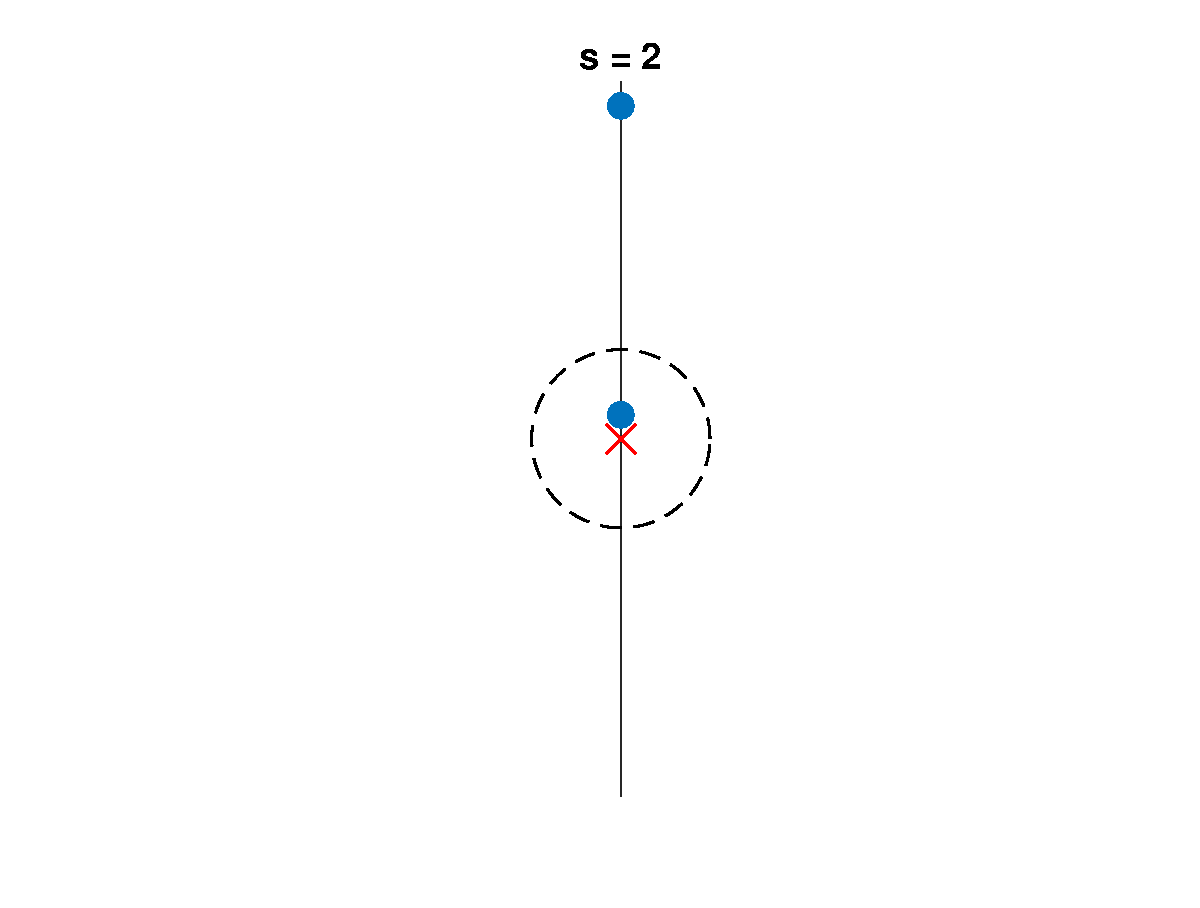
\includegraphics[width=5cm]{images/kreinbubbles/bubble2R} &
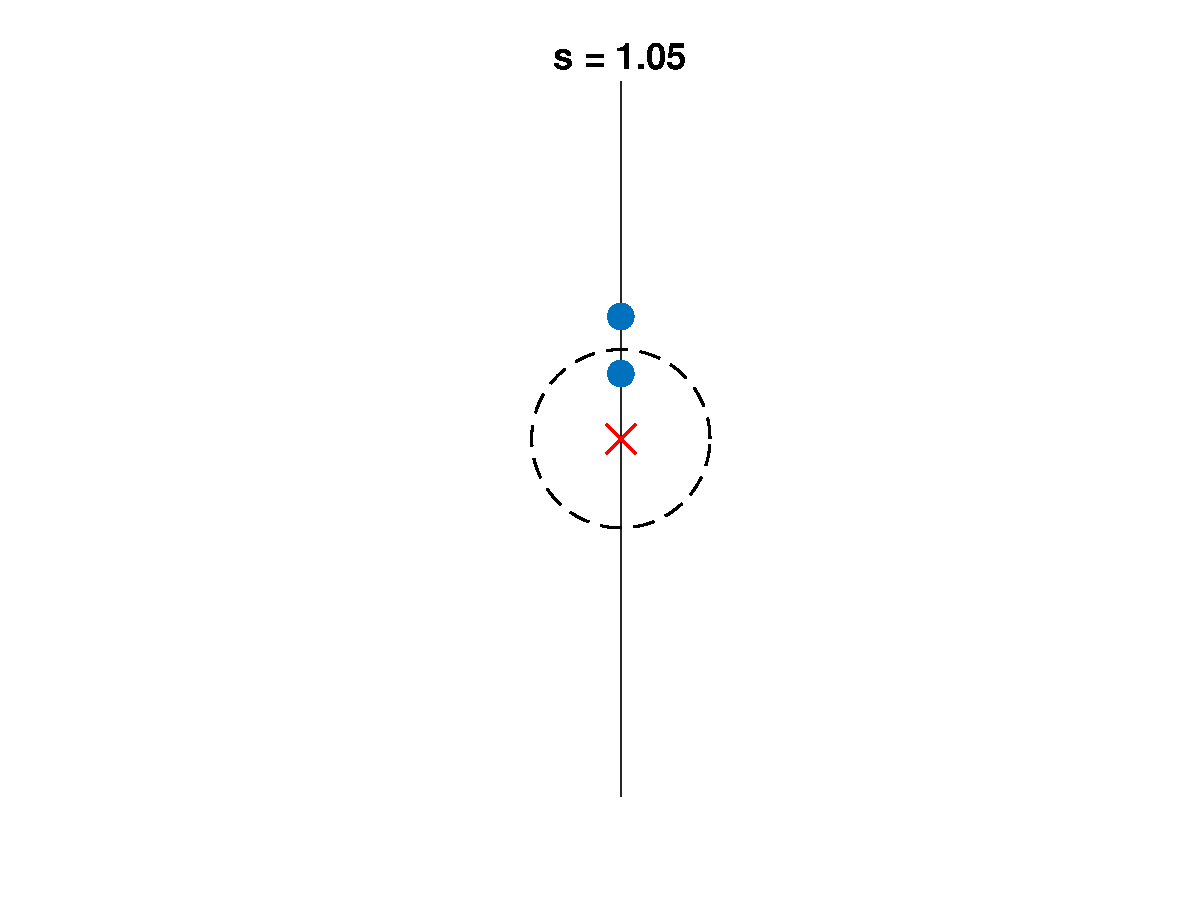
\includegraphics[width=5cm]{images/kreinbubbles/bubble105R} &
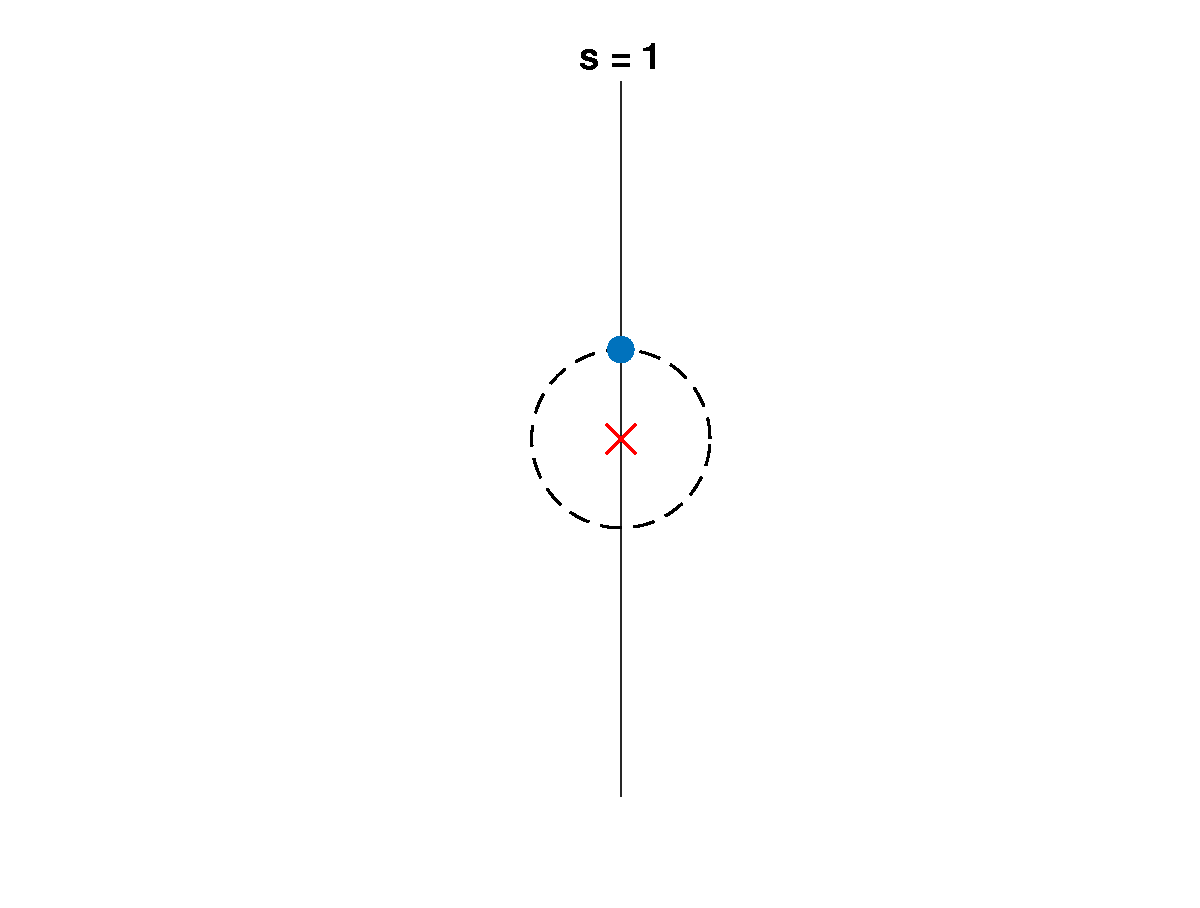
\includegraphics[width=5cm]{images/kreinbubbles/bubbleR} \\
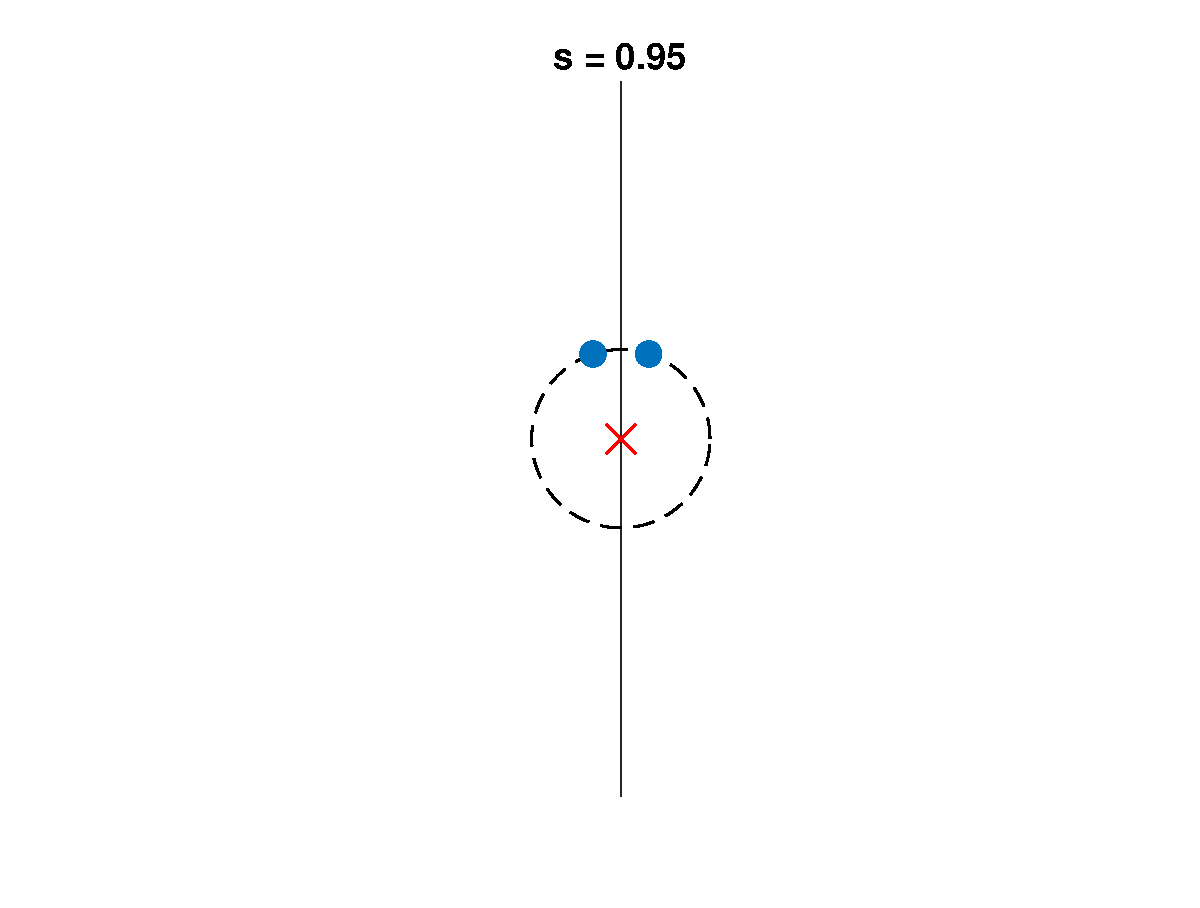
\includegraphics[width=5cm]{images/kreinbubbles/bubble095R} &
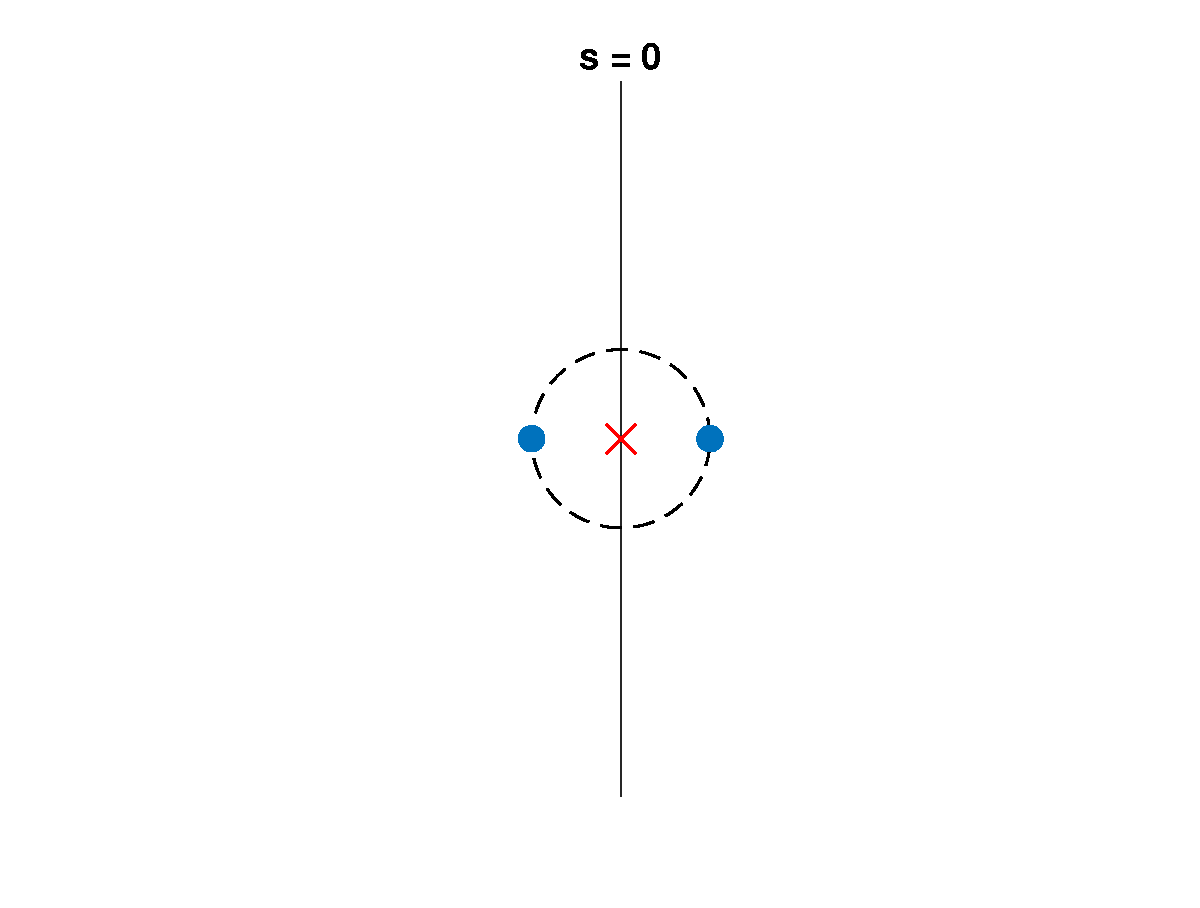
\includegraphics[width=5cm]{images/kreinbubbles/bubble0} &
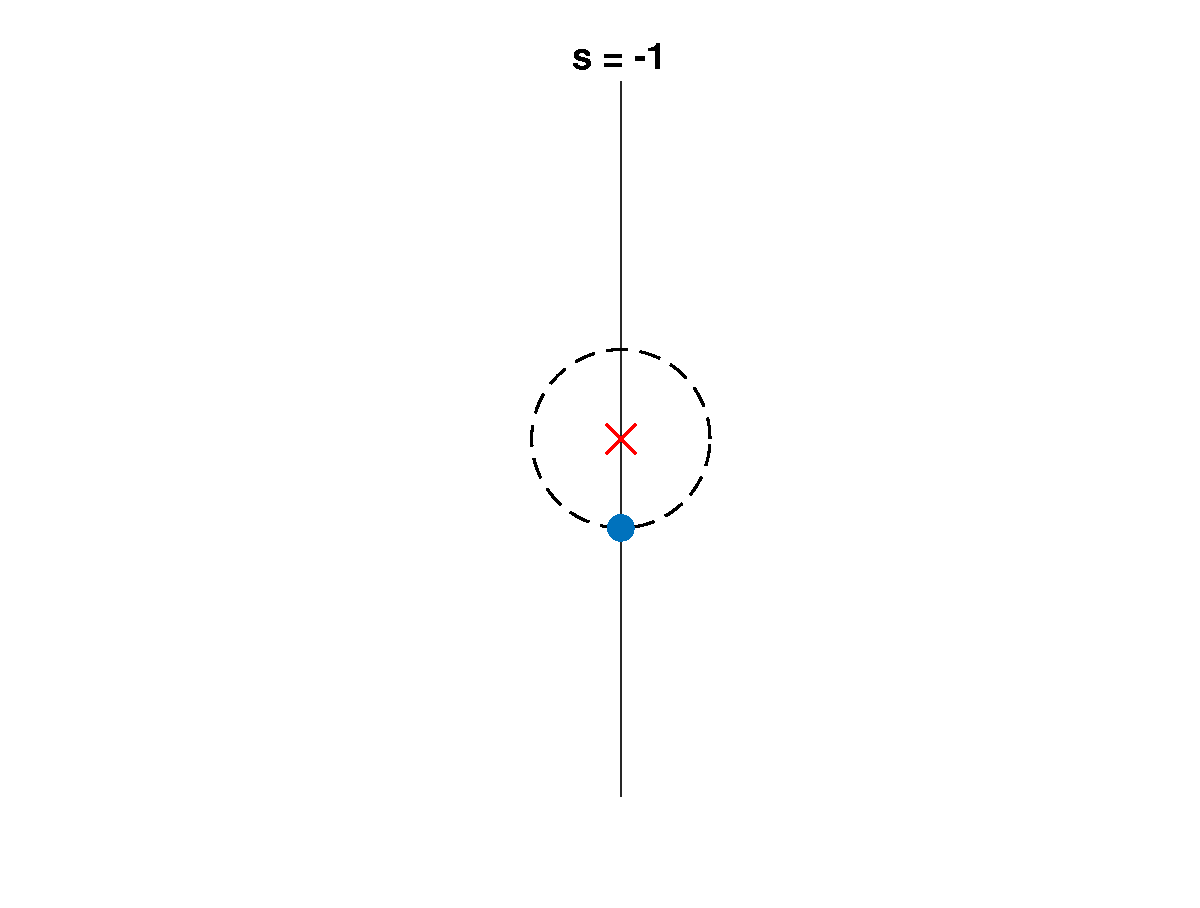
\includegraphics[width=5cm]{images/kreinbubbles/bubbleminusR}
\end{tabular}
\caption{Plot of the complex plane illustrating eigenvalue collision and Krein bubble as parameter $s$ is decreased. Blue dots are the pair of eigenvalues. Red cross is the point $\lambda_* i$. Vertical line is the imaginary axis. Black dotted circle is the circle of radius $\sqrt{R}$ around $\lambda_*$ }
\label{fig:kreinbubbles}
\end{center}
\end{figure}
We will call the instability bubble a Krein bubble, since it results from the collision of two imaginary eigenvalues with opposite Krein signatures. Inside the Krein bubble, the eigenvalues $\lambda_{1,2}$ are symmetric across the imaginary axis. Outside the Krein bubble, there is no such symmetry for $\lambda_{1,2}$; since $\lambda_{1,2}$ are purely imaginary, Hamiltonian symmetry tells that there exist eigenvalues $-\lambda_{1,2}$ which are below the real axis.

In the following theorem, we prove that these Krein bubbles occur. Since the bubbles are formed as $X$ is varied near $X^*$ we will parameterize both $X$ and the eigenvalues $\lambda_{1,2}$ by a single dimensionless parameter $s \in [-2, 2]$. THE ``h.o.t'' WILL BE SPECIFIED ONCE THE PROOF IS COMPLETE. WE COULD ALSO JUST DO THIS FOR $m = 1$.

\begin{theorem}\label{theorem:kreinbubbles}
Let $\delta > 0$ be as in Theorem \ref{blockmatrixtheorem} [Theorem 5.4, the block matrix theorem]. Define
\begin{itemize}
\item $\lambda_m = c \frac{m \pi}{X}$, where $m$ is a positive integer such that $\lambda_m < \delta$.
\item $\lambda_* = \sqrt{\frac{2 a_0}{M}}$
\item $X_m^* = \frac{c m \pi}{\lambda_*}$
\item $R_0 = -\frac{4 p_1 k_0}{M}$ [OR SOMETHING CLOSE TO THIS], where $p_1$, $k_0$, and $M$ are defined in Theorem \ref{blockmatrixtheorem} [Theorem 5.4].
\item $R = \lambda_*^2 R_0 \frac{X_0}{X}$ 
\end{itemize}
Assume $R_0 > 0$. Then there exists $r_1 > 0$ such that for all $r \leq r_1$, the following is true. Let $s \in [-2, 2]$. For $X = X(s)$ close to $X_m^*$, there exists a pair of eigenvalues located at
\begin{align*}
\lambda_{1,2}(s) = \left( \lambda_* + s \sqrt{R} \right) i \pm \sqrt{R(1 - s^2)} + \text{``h.o.t.''}
\end{align*}
where
\[
X(s) = \frac{c m \pi}{s \sqrt{R} + \lambda_*}
\]
and $X(0) = X_m^*$. These eigenvalues have the following configuration.
\begin{itemize}
\item For $|s| < 1$, $\lambda_{1,2}(s)$ is symmetric across the imaginary axis, i.e. $\lambda_2(s) = -\overline{\lambda_1}(s)$. For $s = 0$, these are given by
\[
\lambda_{1,2}(s) = \lambda_* i \pm (\sqrt{R} + ``h.o.t.'')
\]
\item For $|s| \in (1, 2]$, $\lambda_{1,2}(s)$
are purely imaginary. For $s = 2$, one of $\lambda_{1,2}(s)$ is close to $\lambda_* i$.
\item At $s = \pm 1$, $\lambda_{1,2}(s)$ collide on the imaginary axis at 
\[
\lambda_{1,2}(s) = \lambda_* i \pm (\sqrt{R} + ``h.o.t.'')
\]
\end{itemize}
For $|s| \leq 1$, the eigenvalues $\lambda_{1,2}(s)$ are, to leading order, located on a circle of radius $\sqrt{R}$ about $\lambda_* i$ in the complex plane, where
\[
\sqrt{R} = \mathcal{O}\left( r^{3/4}\frac{X_0}{X} \right)
\]
\end{theorem}

\section{Determinant of block matrix}

In this section, we will compute the determinant of the block matrix from \cref{blockmatrixtheorem} for the periodic 2-pulse. This is a $4 \times 4$ matrix, and although the computation is tedious, it can be done with the aid of Mathematica. Before we can do that, we will prove the following bound which makes this computation significantly easier. Since all eigenvalues we will consider have real part of order $\mathcal{O}(r^{1/2})$ or smaller, this is not a restriction.

\begin{lemma}\label{lemma:expnubound}
Let $|\lambda| < \delta$. Then if $|\Re \lambda| \leq C_1 r^{1/2}$ and $r^{1/2} X \leq C_2$, we have the bound
\begin{equation}\label{expnubound}
\left|e^{\nu(\lambda)x}\right| \leq C \\
\end{equation}
for any $x$ with $|x| \leq X$. The constant $C$ only depends on $C_1$, $C_2$, and $\delta$.
\begin{proof}
Let $\lambda = a + bi$ with $|a| \leq C r^{1/2}/X^{1/2}$. Since $|\lambda| \leq \delta$, $|a|, |b| \leq \delta$ as well. Then from Lemma \ref{nulambdalemma},
\begin{align*}
\nu(\lambda) &= \frac{1}{c}\lambda + \mathcal{O}(\lambda^3) \\
&= \frac{a}{c} + i \frac{b}{c} + \mathcal{O}\left( a(a^2 + \delta^2) \right) + i \mathcal{O}\left( a(b^2 + \delta^2) \right)
\end{align*}
where both of the remainder terms are real. (We split the remainder up into real and imaginary parts). Thus 
\begin{align*}
\nu(\lambda)X &= \frac{a}{c}X + i \frac{b}{c}X + \mathcal{O}\left( a(a^2 + \delta^2) X\right) + i \mathcal{O}\left( a(b^2 + \delta^2) X\right)
\end{align*}
When we evaluate $|\exp{(\nu(\lambda)X)}|$, the two imaginary terms on the RHS do not contribute. Since $|a| \leq C_1 r^{1/2}$ and $r^{1/2}X \leq C_2$, 
\begin{align*}
\left| \frac{a}{c}X + \mathcal{O}\left( a(a^2 + \delta^2) X \right) \right| &\leq C(1 + \mathcal{O}(|a|^2 + \delta^2)) \leq C
\end{align*}
where the constant $C$ only depends on $\delta$, $C_1$, and $C_2$. Thus we have
\begin{align*}
|\exp{(\nu(\lambda)X)}| &\leq
\exp{ \left| \frac{a}{c}X + \mathcal{O}\left( a(a^2 + \delta^2) X \right) \right| } \leq C
\end{align*}
The same bound holds for $|x| \leq X$.
\end{proof}
\end{lemma}

In all cases, we will only consider eigenvalues with real part at most $\mathcal{O}(r^{1/2})$. In \cref{section:2pernobubble}, the condition \cref{nobubblecond} guarantees that the hypotheses of \cref{lemma:expnubound} are satisfied. In \cref{section:2perbubble}, we are taking $r^{1/2} X = C$, so the hypotheses of \cref{lemma:expnubound} are also satisfied. 

Using this estimate, we compute the determinant of the block matrix in Theorem \ref{blockmatrixtheorem} for the periodic 2-pulse. Since this is a $4\times 4$ matrix with tons of remainder terms, our only hope is to do this with Mathematica.

\begin{lemma}\label{2blockmatrix}
For $|\lambda| < \delta$ with $|\Re \lambda| \leq C r^{1/2}X^{1/2}$, the determinant of the block matrix $B$ is 
\begin{equation}\label{2detBeq}
\begin{aligned}
\det &B(\lambda, r) = \left(-2 \lambda^2 M (2a + \lambda^2 M) +  \mathcal{O}( (r^{1/2} + |\lambda|)^5 )\right) \sinh(\nu(\lambda)X) \\
&-16 M M^c \lambda^4 ( q(X_0)\sinh(\nu(\lambda)X_0) + q(X_1) \sinh(\nu(\lambda)X_1) ) \cosh(\nu(\lambda)X)  \\
&+ \mathcal{O}( (r^{1/2} + |\lambda|)^6) 
\end{aligned}
\end{equation}
\begin{proof}
First, we write the block matrix $B$ as $B = B_1 + B_2$, where
\[
B_1 = \begin{pmatrix}
\begin{pmatrix}
e^{-\nu(\lambda)X_1} & -e^{\nu(\lambda)X_0} \\
-e^{\nu(\lambda)X_1} & e^{-\nu(\lambda)X_0} 
\end{pmatrix} &
2 \lambda \begin{pmatrix}
-e^{-\nu(\lambda)X_1} q(X_1) + e^{\nu(\lambda)X_0} q(X_1) & e^{-\nu(\lambda)X_1} q(X_1) - e^{\nu(\lambda)X_0} q(X_1) \\ e^{-\nu(\lambda)X_0} q(X_1) - e^{\nu(\lambda)X_1} q(X_1) & -e^{-\nu(\lambda)X_0} q(X_1) + e^{\nu(\lambda)X_1} q(X_1)
\end{pmatrix} \\
-M^c \lambda
\begin{pmatrix}
e^{-\nu(\lambda)X_1} & e^{\nu(\lambda)X_0} \\
e^{\nu(\lambda)X_1} & e^{-\nu(\lambda)X_0} 
\end{pmatrix} &
\begin{pmatrix}
-a - \lambda^2 M & a \\
a & -a - \lambda^2 M
\end{pmatrix}
\end{pmatrix}
\]
and $B_2$ is the block matrix 
\[
B_2 = \begin{pmatrix}
G_1 & G_2 \\ G_3 & G_4
\end{pmatrix}
\]
By our choice of $\lambda$, it follows from \cref{lemma:expnubound} that all the terms of the form $e^{\pm \nu(\lambda)X_j}$ are bounded by a constant. Thus the remainder matrices $G_i$ have bounds
\begin{equation}\label{Gimatrixbounds}
\begin{aligned}
|G_1| &\leq C |\lambda| (|\lambda| + r^{1/2} )\\
|G_2| &\leq C |\lambda| (|\lambda| + r^{1/2} )^2 \\
|G_3| &\leq C (|\lambda| + r^{1/2} )^2 \\
|G_4| &\leq C (|\lambda| + r^{1/2} )^3 \\
\end{aligned}
\end{equation}
We use Mathematica to evaluate the determinant. Briefly, we write the matrices $G_j$ as
\[
G_j = \begin{pmatrix}t^j_1 & t^j_2 \\ t^j_3 & t^j_4 \end{pmatrix}
\]
where the the coefficients $t^j_k$ have bounds given by \cref{Gimatrixbounds}. We then use Mathematica to expand the determinant, and we track each of the $t^j_k$. Doing all of this, we have
\begin{equation}\label{2detB1}
\begin{aligned}
\det &B(\lambda, r) = \sinh(\nu(\lambda)X)\left(-2 \lambda^2 M (2a + \lambda^2 M) +  \mathcal{O}( (r^{1/2} + |\lambda|)^5 )\right) \\
&-4\lambda^4 q(X_0) M M^c \left( \sinh(\nu(\lambda)(2 X_0 + X_1)) - 3 \sinh(\nu(\lambda)X_1)  \right) \\
&-4\lambda^4 q(X_1) M M^c \left( \sinh(\nu(\lambda)(2 X_1 + X_0)) - 3 \sinh(\nu(\lambda)X_0)  \right) \\
&+ \mathcal{O}( (r^{1/2} + |\lambda|)^6) 
\end{aligned}
\end{equation}
Using standard hyperbolic trigonometric identities, we can show that 
\begin{align*}
\sinh(2 x + y) - 3 \sinh(y) &= 4 \cosh(x + y)\sinh(x) 
-2 \sinh(x+y)\cosh(x) 
\end{align*}
Using this with the second line of \cref{2detB1}, 
\begin{align*}
\lambda^4 &q(X_0) \left( \sinh(\nu(\lambda)(2 X_0 + X_1)) - 3 \sinh(\nu(\lambda)X_1)  \right) \\
&= 4 \lambda^4 q(X_0) \cosh(\nu(\lambda)X)\sinh(\nu(\lambda)X_0) - 3 \lambda^4 q(X_0) \sinh(\nu(\lambda)X)\cosh(\nu(\lambda)X_0) \\
&= 4 \lambda^4 q(X_0) \cosh(\nu(\lambda)X)\sinh(\nu(\lambda)X_0) + \sinh(\nu(\lambda)X)(\mathcal{O}(r^{1/2}|\lambda|^4))
\end{align*}
since $|\cosh(\nu(\lambda)X_0)|\leq C$ by Lemma \ref{lemma:expnubound}. Doing the same thing for the third line of \cref{2detB1}, substituting the results into \cref{2detB1}, and simplifying, we have
\begin{equation*}
\begin{aligned}
\det &B(\lambda, r) = \left(-2 \lambda^2 M (2a + \lambda^2 M) + \mathcal{O}( (r^{1/2} + |\lambda|)^5 )\right) \sinh(\nu(\lambda)X) \\
&-16 M M^c \lambda^4 ( k_0\sinh(\nu(\lambda)X_0) + k_1 \sinh(\nu(\lambda)X_1) ) \cosh(\nu(\lambda)X)  \\
&+ \mathcal{O}( (r^{1/2} + |\lambda|)^6) 
\end{aligned}
\end{equation*}
\end{proof}
\end{lemma}

We now have an equation we can solve to find the eigenvalues $\lambda$. However, this equation involves both $\lambda$ and $\nu(\lambda)$, which is annoying. We will simplify the problem by making a change of variables. Since $\nu'(0) = 1/c$ and $\nu(0) = 0$, $\nu(\lambda)$ is invertible near 0. If necessary, decrease $\delta$ so that $\nu(\lambda)$ is invertible for $|\lambda| < \delta$. Let $\lambda = \nu^{-1}(\mu)$. Expanding in Taylor series about $\mu = 0$, we have
\[
\nu^{-1}(\mu) = c \mu + \mathcal{O}(\mu^3)
\]
Substituting this into \cref{2detBeq} and simplifying, 
\begin{equation}\label{2detBeqmu}
\begin{aligned}
\det &B(\mu, r) = \left(-2 c^2 \mu^2 M (2a + c^2 \mu^2 M) +  \mathcal{O}( (r^{1/2} + |\mu|)^5 )\right) \sinh(\mu X) \\
&+16 p_1 M c^4 \mu^4 ( k_0\sinh(\mu X_0) + k_1 \sinh(\mu X_1) ) \cosh(\mu X)  \\
&+ \mathcal{O}( (r^{1/2} + |\mu|)^6) 
\end{aligned}
\end{equation}
To find the eigenvalues, we will find the zeros of \cref{2detBeqmu}. We will do this for several specific cases.

\section{Computation of coefficients $a_j$}

Next, we compute the coefficients $a_j$ of the matrix $A$ in lower right block of the block matrix equation.

\begin{lemma}\label{lemma:ajparam}
For the coefficients $a_j$ in the block matrix equation, 
\begin{equation}\label{ajparam}
a_j = s_0 e^{\alpha \phi/\beta} r b_j \left( \beta \cos\left(-\rho \log b_j \right) - \alpha \sin \left(-\rho \log b_j \right) \right) + \mathcal{O}(r^{1+\gamma/2\alpha})
\end{equation}

\begin{proof}
From \cite[Lemma 6.1]{Sandstede1998},
\begin{align*}\label{IPpsiQprime}
\langle \Psi(-x), Q'(x) \rangle
&= s_0 e^{-2 \alpha x}\left( \beta \cos(2 \beta x + \phi) - \alpha \sin(2 \beta x + \phi)\right) + \mathcal{O}(e^{-(2 \alpha + \gamma) x}
\end{align*}
where $s_0 > 0$ and $\gamma$ are the same as in Lemma \ref{IPform}. Thus we have
\begin{align*}
a_j &= \langle \Psi(-X_j), Q'(X_j) \rangle \\
&= s_0 e^{-2 \alpha X_j}\left( \beta \cos(2 \beta X_j + \phi) - \alpha \sin(2 \beta X_j + \phi)\right) + \mathcal{O}(e^{-(2 \alpha + \gamma) X_j}) \\
&= s_0 e^{\alpha \phi/\beta} r b_j \left( \beta \cos\left( -\frac{\beta}{\alpha} \log(b_j r) \right) - \alpha \sin \left( -\frac{\beta}{\alpha} \log(b_j r) \right) \right) + \mathcal{O}(r^{1+\gamma/2\alpha} b_j^{1 + \gamma/2\alpha}) \\
&= s_0 e^{\alpha \phi/\beta} r b_j \left( \beta \cos\left( -\rho \log(b_j r) \right) - \alpha \sin \left( -\rho \log(b_j r) \right) \right) + \mathcal{O}(r^{1+\gamma/2\alpha})
\end{align*}
since $b_j \in (0, 1]$. Since $r \in \mathcal{R}$, $r = \exp\left(-\frac{2 m \pi}{\rho}\right)$ for some nonnegative integer $m$, this becomes 
\begin{align*}
a_j &= s_0 e^{\alpha \phi/\beta} r b_j \left( \beta \cos\left( 2 m \pi -\rho \log b_j \right) - \alpha \sin \left( 2 m \pi -\rho \log b_j \right) \right) + \mathcal{O}(r^{1+\gamma/2\alpha}) \\
&= s_0 e^{\alpha \phi/\beta} r b_j \left( \beta \cos\left(-\rho \log b_j \right) - \alpha \sin \left(-\rho \log b_j \right) \right) + \mathcal{O}(r^{1+\gamma/2\alpha})
\end{align*}
\end{proof}
\end{lemma}

In the next sections, we will prove \cref{theorem:2peigscase1}. First, we locate the eigenvalues at 0.

\section{Eigenvalues at 0}

The corresponding eigenfunctions are $\partial_x Q_2(x)$ and $\partial_c Q_2(x)$. We will show that there is one more eigenvalue at 0.

Start with equation \cref{2detBeqmu}. Let $\mu_*(r) = \sqrt{-2a(r)/M c^2}$. By \cref{lemma:expnubound}, all the $\sinh$ and $\cosh$ terms in \cref{2detBeqmu} are bounded by a constant. Since $q(X_j) = \mathcal{O}(r^{1/2})$, equation \cref{2detBeqmu} simplifies to
\begin{equation}\label{2detBeqmu3}
\begin{aligned}
\det B(\mu, r) &= -2 \mu^2 M (\mu - \mu_*(r)) (\mu + \mu_*(r)) \sinh(\mu X) + \mathcal{O}( r^{1/2} + |\mu|)^5
\end{aligned}
\end{equation}
By the condition \cref{nobubblecond}, $\mu X \leq 1/2$, thus we expand the $\sinh(\mu X)$ term in a Taylor series about 0 to get
\begin{equation}\label{2detBeqmu4}
\begin{aligned}
\det B(\mu, r) &= -2 \mu^2 M (\mu - \mu_*(r)) (\mu + \mu_*(r))( \mu X + \mathcal{O}(\mu X)^3) + \mathcal{O}( r^{1/2} + |\mu|)^5
\end{aligned}
\end{equation}
Finally, rescale the problem by taking
\begin{align*}
\mu = r^{1/2}\tilde{\mu} \\
\mu_*(r) = r^{1/2}\tilde{\mu}_*(r)
\end{align*}
Substituting these in, we have
\begin{equation}\label{2detBeqmu5}
\begin{aligned}
\det B(\tilde{\mu}, r) &= -2 \tilde{\mu}^2 M r^{5/2} (\tilde{\mu} - \tilde{\mu}_*(r)) (\tilde{\mu} + \tilde{\mu}_*(r))( \tilde{\mu} X + \mathcal{O}(\tilde{\mu}^3 r X^3) + \mathcal{O}( r^{1/2} + |\mu|)^5
\end{aligned}
\end{equation}
By \cref{lemma:ajparam}, $\tilde{\mu}_*(r) = \tilde{\mu}_*(0) + \mathcal{O}(r^{\gamma/4 \alpha)}$, thus we have
\begin{equation}\label{2detBeqmu5}
\begin{aligned}
\det B(\tilde{\mu}, r) &= -2 \tilde{\mu}^2 M r^{5/2} (\tilde{\mu} - \tilde{\mu}_*(0)) (\tilde{\mu} + \tilde{\mu}_*(0))( \tilde{\mu} X + \mathcal{O}(\tilde{\mu}^3 r X^3) + \mathcal{O}( r^{1/2} + |\mu|)^5
\end{aligned}
\end{equation}

We want to show that $\det B(\mu, r)$ has exactly three zeros inside a small circle around the origin in the complex plane. To do this, consider a circle of radius $\xi$, where
\[
\xi = \frac{1}{2}|\mu_*(0)|
\]
Then for $\mu$ with $|\mu| = \xi$,
\begin{equation*}
\begin{aligned}
\det B(\tilde{\mu}, r) &= -2 \tilde{\mu}^2 M r^{5/2} (\tilde{\mu} - \tilde{\mu}_*(0)) (\tilde{\mu} + \tilde{\mu}_*(0))( \tilde{\mu} X + \mathcal{O}(\tilde{\mu}^3 r X^3) + \mathcal{O}( r^{5/2} )
\end{aligned}
\end{equation*}
Dividing by $r^{5/2}X$ and recalling that $X = \mathcal(|\log r|)$, we are looking for zeros of
\[
G(\tilde{\mu}, r) = -2 \tilde{\mu}^3 M (\tilde{\mu} - \tilde{\mu}_*(0)) (\tilde{\mu} + \tilde{\mu}_*(0)) + \mathcal{O}\left( r |\log r|^2 + \frac{1}{|\log r|} \right)
\]
which we write as $G(\tilde{\mu}, r) = G_1(\tilde{\mu}) + G_2(\tilde{\mu}, r)$, where 
\[
G_1(\tilde{\mu}) = -2 \tilde{\mu}^3 M (\tilde{\mu} - \tilde{\mu}_*(0)) (\tilde{\mu} + \tilde{\mu}_*(0)),
\]
which is independent of $r$, and
\[
G_2(\tilde{\mu}, r) = \mathcal{O}\left( r |\log r|^2 + \frac{1}{|\log r|} \right)
\]

Let $\xi = r^{1/2} \tilde{\xi} = \tilde{\mu}_*(0)/2|$. Then on a circle of radius $\tilde{\xi}$,
\[
|G_1(\tilde{\mu})| \geq \frac{|M|}{16}|\tilde{\mu}_*(0)|^5
\]
Since $|G_2(\tilde{\mu}, r)| \rightarrow 0$ as $r \rightarrow 0$, as long as $\tilde{\mu}_*(0) \neq 0$, there exists $r_1 \leq r_0$ such that $|G_2(\tilde{\mu}, r)| < |G_1(\tilde{\mu})|$ on a circle of radius $\tilde{\xi}$. By Rouch\'{e}'s theorem $G(\tilde{\mu}, r)$ and $G_1(\tilde{\mu})$ have the same number of zeros (counted with multiplicity) inside the circle of radius $\tilde{\xi}$. By the choice of $\tilde{\xi}$, $G_1(\tilde{\mu})$ has exactly 3 zeros inside the circle, thus $G(\tilde{\mu}, r)$ does as well. Since there is an eigenvalue at 0 of at least algebraic multiplicity 2, at least two of these zeros must be at the origin. By Hamiltonian symmetry, the third zero must also be at the origin.

\section{Essential spectrum eigenvalues}

In this section, we will look for the essential spectrum eigenvalues. We will only do this for Case 1. In terms of $\mu$, we expect to find the essential spectrum eigenvalues near $\pm m \pi i/X$ for integer $k$. Let $r_0$ be as above, and for $r = r_0$, let $M$ be the largest integer such that $\left| c \frac{M \pi}{X} \right| < \delta$. Let $m$ be a nonzero integer with $|m| \leq M$, and let
\[
\mu_m = \frac{m \pi i}{X} + \frac{h}{X}
\]
Expanding the $\sinh(\mu_m X)$ and $\cosh(\mu_m X)$ terms in \cref{2detBeqmu} about $m \pi/X$, we have
\begin{align*}
\sinh(\mu_m X) &= (-1)^m h + \mathcal{O}(h^3) \\
\cosh(\mu_m X) &= (-1)^m + \mathcal{O}(h^2) \\
\end{align*}
By \cref{lemma:expnubound}, the $\sinh(\mu_m X_j)$ terms in \cref{2detBeqmu} are bounded by a constant. The $k_j$ terms are $\mathcal{O}(r^{1/2})$. By the assumptions in Case 1, $|\mu_m| \geq C r^{1/2}$. Substituting these into \cref{2detBeqmu}, we have 
\begin{equation}\label{Bess1}
\begin{aligned}
\det &B(h, r) = \left(-2 c^2 M  \mu_m^2 \left( 2a + c^2 M \mu_m \right)^2 + \mathcal{O}( |\mu_m|)^5 \right) \left( (-1)^m h + \mathcal{O}(h^3) \right) \\
&+ \mu_m^4 \left( (-1)^m + \mathcal{O}(h^2)\right)\mathcal{O}(r^{1/2}) + \mathcal{O}\left( |\mu_m| \right)^6 \\
&= \left(-2 c^2 M  \mu_m^2 \left( 2a + c^2 M \mu_m \right)^2 + \mathcal{O}( |\mu_m|)^5 \right) \left( (-1)^m h + \mathcal{O}(h^3) \right) + \mathcal{O}\left( |\mu_m|^4(r^{1/2} + |\mu_m|) \right)
\end{aligned}
\end{equation}
We want to solve $\det B(\mu, r) = 0$. To simplify, let $\mu_* = \sqrt{-\frac{2a}{M c^2}}$. Dividing by $(-1)^m$, $M c^2$, and the constants out front, we want to solve 
\begin{equation}\label{Bess2}
\begin{aligned}
\left(\mu_m^2 (\mu_m - \lambda_*)(\mu_m + \lambda_*) + \mathcal{O}( |\mu_m|)^5 \right) \left( h + \mathcal{O}(h^3) \right) + \mathcal{O}\left( |\mu_m|^4(r^{1/2} + |\mu_m|) \right) = 0
\end{aligned}
\end{equation}
Since $\mu_m \neq 0$, divide by $\mu_m^2$ to get
\begin{equation}\label{Bess3}
\begin{aligned}
\left((\mu_m - \lambda_*)(\mu_m + \lambda_*) + \mathcal{O}( |\mu_m|)^3 \right) \left( h + \mathcal{O}(h^3) \right) + \mathcal{O}\left( |\mu_m|^2(r^{1/2} + |\mu_m|) \right) = 0
\end{aligned}
\end{equation}
Finally, multiply by $X^2$ and substitute for $\mu_m$. Since $m \leq M$, simplify the remainder terms to get $F_m(h, r) = 0$, where
\begin{equation}\label{Bess4}
\begin{aligned}
F_m(h, r) &= (m \pi i + h - \lambda_* X)(m \pi i + h + \lambda_* X) \left( h + \mathcal{O}(h^3) \right) + \mathcal{O}\left( r^{1/2} + \frac{1}{X} \right)
\end{aligned}
\end{equation}
Since $X = \mathcal{O}(1/\log|r|)$, $F(0,0) = 0$. Since $\lambda_* = \mathcal{O}(r^{1/2})$, $\lambda_* X \rightarrow 0$ as $r \rightarrow 0$. Thus we have
\[
\partial_h F(0,0) = -m^2 \pi^2
\]
For all $m$ between 1 and $M$, $|\partial_h F(0,0)| \geq \pi^2 > 0$. Thus we can use the implicit function theorem to solve for $h$ in terms of $r$ near $h = 0$. Specifically, there exists $r_1^m \leq r_0$ and a unique smooth function $h_m(r)$ with $h_m(0) = 0$ such that for all $r \leq r_1^m$, $G(h_m(r),r) = 0$. Expanding $h_m$ in a Taylor series about $r = 0$, we have for all $|m| \leq M$,
\[
h_m(r) = \mathcal{O}\left( r^{1/2} + \frac{1}{X} \right)
\]
Do this for all $|m| \leq M$, and let $r_1 = \min\{ r_1^m \}$. Undoing the scaling, for all $r \leq r_1$ and for all nonzero integers $m$ with $|m| \leq M$, there are essential spectrum eigenvalues located at
\[
\mu_m = \frac{m \pi i}{X} + \mathcal{O}\left( \frac{1}{X}\left( r^{1/2} + \frac{1}{X} \right) \right)
\]
Changing variables back to $\lambda$, these are located at
\[
\lambda_m = \frac{m \pi i}{X}\left[1 + \mathcal{O}\left( \frac{1}{X}\left( r^{1/2} + \frac{1}{X} \right) \right) \right] + \mathcal{O}\left( \frac{1}{X}\left( r^{1/2} + \frac{1}{X} \right) \right)
\]
By Hamiltonian symmetry, eigenvalues must come in quartets. Thus $\lambda_m$ is pure imaginary and $\lambda_{-m} = \lambda_m$. We conclude that the nonzero essential spectrum eigenvalues are given by $\lambda = \pm \lambda_m^{\text{ess}}$, where
\[
\lambda_m^{\text{ess}} = \frac{m \pi i}{X}\left[1 + \mathcal{O}\left( \frac{1}{X}\left( r^{1/2} + \frac{1}{X} \right) \right) \right] + \mathcal{O}\left( \frac{1}{X}\left( r^{1/2} + \frac{1}{X} \right) \right)
\]
is pure imaginary. This proves \cref{theorem:2peigscase1} part (ii).

\section{Interaction eigenvalues}

In this section, we will set up the estimates we need for parts (i) and (iii) of \cref{theorem:2peigscase1}. In both cases, we are looking for eigenvalue $\lambda$ of order $r^{1/2}$. Thus \cref{2detBeqmu} simplifies to
\begin{equation}\label{2detBint1}
\begin{aligned}
\det &B(\mu, r) = \left(-2 c^2 \mu^2 M (2a + c^2 \mu^2 M) +  \mathcal{O}( r^{5/2} )\right) \sinh(\mu X) \\
&+16 p_1 M c^4 \mu^4 ( k_0\sinh(\mu X_0) + k_1 \sinh(\mu X_1) ) \cosh(\mu X) + \mathcal{O}( r^3 ) 
\end{aligned}
\end{equation}
For Case 1, $\lambda X \leq c/2$, thus $\mu X \leq 1/2$. We expand the $\sinh$ and $\cosh$ terms in a Taylor series about 0 to get
\begin{align*}
\sinh(\mu X) &= \mu X + \mathcal{O}\left(\mu X \right)^3 \\
\cosh(\mu X) &= 1 + \mathcal{O}\left(\mu X\right)^2 \\
\sinh(\mu X_j) &= \mu X_j + \mathcal{O}\left(\mu X_j \right)^3
\end{align*}
Substituting these and simplifying, we obtain 
\begin{equation}\label{2detBint2}
\begin{aligned}
\det &B(\mu, r) = \left(-2 c^2 \mu^2 M (2a + c^2 \mu^2 M) +  \mathcal{O}( r^{5/2} )\right) \left(\mu X + \mathcal{O}\left(\mu X \right)^3 \right) \\
&+16 p_1 M c^4 \mu^4 \left( k_0\left( \mu X_0 + \mathcal{O}(\mu X_0)^3 \right)  + k_1\left( \mu X_1 + \mathcal{O}(\mu X_1) ^3 \right) \right) \left( 1 + \mathcal{O}(\mu X)^2 \right) \\
&+ \mathcal{O}( r^3 )
\end{aligned}
\end{equation}
Since $k_j$ terms are $\mathcal{O}(r^{1/2})$, this simplifies to 
\begin{equation}\label{2detBint2}
\begin{aligned}
\det &B(\mu, r) = -2 c^2 \mu^2 M (2a + c^2 \mu^2 M)\left( \mu X + \mathcal{O}\left(\mu X \right)^3 \right)
+ \mathcal{O}( r^3 X ) 
\end{aligned}
\end{equation}
We wish to solve the equation $\det B(\mu, r) = 0$. Next, we scale out the scaling parameter $r$ from the eigenvalues. Let $\mu = r^{1/2}\tilde{\mu}$ and $a = r \tilde{a}(r) = r (\tilde{a}_1(r) + \tilde{a}_2(r))$. From Lemma \ref{lemma:ajparam}, 
\begin{align}\label{tildea1}
\tilde{a}_j(r) &= s_0 e^{\alpha \phi/\beta} b_j(r) \left( \beta \cos\left(-\rho \log b_j(r) \right) - \alpha \sin \left(-\rho \log b_j(r) \right) \right) + \mathcal{O}(r^{1+\gamma/2\alpha})
\end{align}
Making this substitution and dividing by $r^{5/2}$ and the constants out front, we want to solve
\begin{equation}\label{2detBint4}
\begin{aligned}
\tilde{\mu}^2 (2\tilde{a}(r) + c^2 \tilde{\mu}^2 M)\left( \tilde{\mu} X + \mathcal{O}(r X^3)\right) + \mathcal{O}( r^{1/2} X ) = 0
\end{aligned}
\end{equation}
Let $\tilde{\mu}_*(r) = \sqrt{-\frac{2\tilde{a}(r)}{M c^2}}$. Dividing by $X$ and $c^2 M$ and simplifying, we wish to solve $G(\tilde{\mu},r) = 0$, where
\begin{equation}\label{2detBint4}
\begin{aligned}
G(\tilde{\mu},r) = \tilde{\mu}^2 (\tilde{\mu} - \tilde{\mu}_*(r))(\tilde{\mu} + \tilde{\mu}_*(r))\left( \tilde{\mu} + \mathcal{O}(r X^2)\right) + \mathcal{O}( r^{1/2} ) = 0
\end{aligned}
\end{equation}
We expect to have interaction eigenvalues near $\tilde{\mu} = \pm \tilde{\mu}_*(r)$. We will look near $\tilde{\mu}_*(r)$ first. Let
\[
\tilde{\mu} = \tilde{\mu}_*(r) + \tilde{h}
\]
Then \cref{2detBint4} becomes
\begin{equation}\label{2detBint5}
\begin{aligned}
G(\tilde{h},r) = \tilde{h} ( \tilde{h} + \tilde{\mu}_*(r))^2 (\tilde{h} + 2 \tilde{\mu}_*(r))\left(\tilde{h} + \tilde{\mu}_*(r) + \mathcal{O}(r X^2)\right) + \mathcal{O}( r^{1/2} ) = 0
\end{aligned}
\end{equation}
Taking the derivative with respect to $\tilde{h}$ at $\tilde{h} = 0$, we have
\[
\partial_{\tilde{h}} G(0, 0) = 2 \tilde{\mu}_*(0)^4 
\]
which is 0 if and only if $\tilde{a}(0) = 0$. As long as we avoid that, we can use the implicit function theorem. We will now prove a result giving a criterion for when $\tilde{a}(0) = 0$.

\begin{lemma}\label{lemma:tildea0zero}
$\tilde{a}_0 = 0$ if and only if the 2-pulse $Q_2(x)$ is parameterized by $b^*_0(0) = b^*_1(0) = p_k^*$, where $p_k^*$ is one of the pitchfork bifurcation points in the limiting case where $r = 0$.
\begin{proof}
For convenience, let $b^*_j = b^*_j(0)$. From \cref{tildea1},
\begin{align}\label{tildear}
\tilde{a}_j(r) &= s_0 e^{\alpha \phi/\beta} b^*_j \left( \beta \cos\left(-\rho \log b^*_j \right) - \alpha \sin \left(-\rho \log b^*_j \right) \right) + + \mathcal{O}(r^{\gamma/2\alpha})
\end{align}
thus we have
\begin{align}\label{tildea0}
\tilde{a}(0) &= s_0 e^{\alpha \phi/\beta}\left[ b^*_0 ( \beta \cos(-\rho \log b^*_0 ) - \alpha \sin (-\rho \log b^*_0 )  + b^*_1 ( \beta \cos(-\rho \log b^*_1 ) - \alpha \sin (-\rho \log b^*_1 ) \right]
\end{align}
Recall from the construction of the periodic 2-pulse that
\begin{equation}\label{b0b1relation}
b^*_0 \sin (-\rho \log b^*_0) = b^*_1 \sin(-\rho \log b^*_1)
\end{equation}
BY A TEDIOUS COMPUTATION WHICH IS NOT YET DONE BUT VERY STRONGLY SUGGESTED BY NUMERICS, the only solution to $\tilde{a}(0) = 0$ which satisfies \cref{b0b1relation} is given by 
\[
b_0^* = b_1^* = p_k^*
\]
for integer $k$, where $p_k^*$ is one of the pitchfork bifurcation points in the zero set of $H(b^*_0, b^*_1)$ from Lemma \ref{pitchforkH}.
\end{proof}
\end{lemma}

Since the pitchfork bifurcation points only happen along the diagonal, we will consider the cases of asymmetric and symmetric periodic 2-pulses separately.

\subsection{Asymmetric periodic 2-pulses}

In the asymmetric case, if $X_1 > X_0$, then $b^*_0(0) \neq b^*_1(0)$. By \cref{lemma:tildea0zero}, $\tilde{a}_0 \neq 0$, thus $\tilde{\mu}_*(0) \neq 0$. Thus we can use the implicit function theorem to solve \cref{2detBint5} for $\tilde{h}$ in terms of $r$ near $\tilde{h} = 0$. Specifically, there exists $r_1 \leq r_0$ and a unique smooth function $\tilde{h}$ with $\tilde{h}(0) = 0$ such that for all $r \leq r_1$, $G(\tilde{h}, r) = 0$. Expanding $\tilde{h}$ in a Taylor series about $r = 0$, we have
for all $r \leq r_1$,
\[
\tilde{h} = \mathcal{O}( r^{1/2} )
\]
Undoing the scaling, for all $r \leq r_1$, there is an interaction eigenvalue located at
\begin{align*}
\mu^+(r) = \sqrt{-\frac{2 a(r)}{M c^2}} + \mathcal{O}(r)
\end{align*}
Changing variables back to $\lambda$, this is located at
\begin{align*}
\lambda^+(r) = \sqrt{-\frac{2 a(r)}{M}} + \mathcal{O}( r )
\end{align*}
Similarly, if we let $\tilde{\mu} = -\tilde{\mu}_*(r) + \tilde{h}$, we can find an interaction eigenvalue at
\begin{align*}
\lambda^-(r) = -\sqrt{-\frac{2 a(r)}{M}} + \mathcal{O}( r )
\end{align*}

By Hamiltonian symmetry, eigenvalues must come in quartets. Since there are no more eigenvalues of this magnitude, we conclude that there is a pair of interaction eigenvalues which are either real or pure imaginary and are given by
\[
\lambda^{\text{int}} = \pm \left( \sqrt{-\frac{2 a}{M}} + \mathcal{O}( r^{1/2} ) \right)
\]
This proves \cref{theorem:2peigscase1} part (i).

\subsection{Symmetric periodic 2-pulses}

The final case to consider is the symmetric periodic 2-pulse. In this case, the baseline length parameters are $b_0^0 = b_0^0$, which are either $1$ or $e^{-\frac{1}{\rho} \pi}$. Thus from \cref{thetaparamlemma}, the length parameters are
\[
b_0^*(m, \theta) = b_1^*(m, \theta) = e^{-\frac{1}{\rho}(m \pi - \theta) }
\]
where either $m = 0$ or $m = 1$. Since $\tilde{a}_0 = \tilde{a}_1$, we substitute these into the expression \cref{tildear} to get 
\begin{align*}
\tilde{a}(r) &= 2 s_0 e^{\alpha \phi/\beta} e^{-\frac{1}{\rho}(m \pi - \theta) } \left( \beta \cos\left(-\rho \log e^{-\frac{1}{\rho}(m \pi - \theta) } \right) - \alpha \sin \left(-\rho \log e^{-\frac{1}{\rho}(m \pi - \theta) } \right) \right) + \mathcal{O}(r^{\gamma/2\alpha}) \\
&= s_0 e^{\alpha \phi/\beta} e^{-\frac{1}{\rho}(m \pi - \theta) } \left( \beta \cos\left( m \pi - \theta \right) - \alpha \sin \left( m \pi - \theta \right) \right) + \mathcal{O}(r^{\gamma/2\alpha}) \\
&= (-1)^m s_0 e^{\alpha \phi/\beta} e^{-\frac{1}{\rho}(m \pi - \theta) } \left( \beta \cos \theta + \alpha \sin \theta \right) + \mathcal{O}(r^{\gamma/2\alpha}) 
\end{align*}
When $r = 0$, 
\begin{align*}
\tilde{a}(r) &= (-1)^m s_0 e^{\alpha \phi/\beta} e^{-\frac{1}{\rho}(m \pi - \theta) } \left( \beta \cos \theta + \alpha \sin \theta \right)
\end{align*}
which is 0 if and only if $\beta \cos \theta + \alpha \sin \theta = 0$, i.e.
\[
\theta = -\arctan \rho
\]
At this value of $\theta$,
\[
b_0^*(m, \theta) = b_1^*(m, \theta)= e^{-\frac{1}{\rho}(m \pi - \theta)} = p^*_m
\]
where $p^*_m$ is the pitchfork bifurcation point for the zero set of $H(b_0, b_1)$ when $r = 0$. This is consistent with \cref{lemma:tildea0zero}. 

If $\mu_*(0) \neq 0$, which occurs if $\theta \neq -\arctan \rho$, we can solve for the interaction eigenvalues using the implicit function theorem exactly as in the previous section. We are interested in what happens in a neighborhood of this point.

For simplicity, take the case where $m_0 = m_1 = 0$, and let $\epsilon = \mu_*(0)$. Then in a small neighborhood of $\theta = -\arctan \rho$,
\begin{align*}
\epsilon &< 0 && \theta < -\arctan \rho \\
\epsilon &= 0 && \theta = -\arctan \rho \\
\epsilon &> 0 && \theta = -\arctan \rho 
\end{align*}
Write \cref{2detBint4} as
\begin{equation}\label{2detBintBif}
\begin{aligned}
G(\tilde{\mu},\epsilon, r) = \tilde{\mu}^2 (\tilde{\mu} - \epsilon)(\tilde{\mu} + \epsilon)\left( \tilde{\mu} + \mathcal{O}(r X^2)\right) + \mathcal{O}( r^{1/2} ) = 0
\end{aligned}
\end{equation}
THIS IS BASICALLY THE NORMAL FORM OF A SADDLE EXCEPT IT IS MULTIPLIED BY AN EXTRA $\tilde{\mu}^3$. I ASSUME WE CANNOT JUST DIVIDE BY $\tilde{\mu}^3$ HERE SINCE EVERYTHING IS COLLIDING AT 0.

\section{Krein bubble}

Finally, we look at Case 2, where a purely imaginary interaction eigenvalue is close to an essential spectrum eigenvalue. Let
\[
\mu_m = \frac{m \pi}{X},
\]
where $m$ is a positive integer chosen so that that $c \mu_m < \delta$. Let 
\begin{equation}\label{kreinmustar}
\mu_*(r) = \sqrt{\frac{2 a(r)}{M c^2}} > 0
\end{equation}
so that we expect to find interaction eigenvalues close to $\pm \mu_*(r) i$. Let
\[
X_m^* = \frac{m \pi}{\mu_*}
\]
Since we are looking for eigenvalues close to $\lambda_* = \mathcal{O}(r^{1/2})$, we start with \cref{2detBint1}. Since we are looking for nonzero eigenvalues, we divide by $\mu^2$ and the constants out front to get the equation
\begin{equation}\label{KreinB1}
\begin{aligned}
0 &= \left( (2a(r) + c^2 \mu^2 M) +  \mathcal{O}( r^{3/2} )\right) \sinh(\mu X) \\
&-8 p_1 c^2 \mu^2 ( k_0\sinh(\mu X_0) + k_1 \sinh(\mu X_1) ) \cosh(\mu X) + \mathcal{O}( r^2 ) 
\end{aligned}
\end{equation}
Dividing by $M c^2$ and using \cref{kreinmustar}, this becomes
\begin{equation}\label{KreinB2}
\begin{aligned}
0 &= \left( (\mu - \mu_*(r) i)( \mu + \mu_*(r) i) +  \mathcal{O}( r^{3/2} )\right) \sinh(\mu X) \\
&-\frac{8 p_1}{M} \mu^2 ( k_0\sinh(\mu X_0) + k_1 \sinh(\mu X_1) ) \cosh(\mu X) + \mathcal{O}( r^2 ) 
\end{aligned}
\end{equation}

We will parameterize the system in terms of two parameters: the difference $h$ between $\mu$ and $\mu_*(0)$ and the distance $s$ along the imaginary axis between $\mu_*(0)$ and $\mu_m$. We will only consider the upper half of the complex plane here; what happens in the lower half is the same by Hamiltonian symmetry. Let 
\begin{align*}
h &= \mu - \mu_*(r) i \\
s &= \mu_m - \mu_*(r)
\end{align*}
where $h \in \C$ and $s \in \R$. We will scale $s$ so that it is dimensionless at the end. Our goal is derive a relationship between $s$ and $h$. In order to expand the $\sinh(\mu X)$ and $\cosh(\mu X)$ terms around $\mu_m$, we write $\mu$ as
\begin{align*}
\mu &= \mu - \mu_m i + \mu_m i \\
&= (\mu_*(r) - \mu_m)i + h + \mu_m i \\
&= \mu_m i + s i + h
\end{align*}
Using these, we have the Taylor expansions
\begin{align*}
\sinh(\mu X) &= \sinh((\mu_m + s i + h)X)
= (-1)^m(s i + h)X + \mathcal{O}\left( (s i +h)^3 X^3 \right) \\
\cosh(\mu X) &= \cosh((\mu_m + s i + h)X)
= (-1)^m + \mathcal{O}\left( (s i + h)^2 X^2 \right) \\
\end{align*}
Substituting all of these into \cref{KreinB2}, we obtain the equation
\begin{equation}\label{KreinB3}
\begin{aligned}
0 &= \left( h ( h + 2 \mu_*(r) i) +  \mathcal{O}( r^{3/2} )\right) \left( (-1)^m(s i + h)X + \mathcal{O}\left( (si+h)^3 X^3 \right)  \right) \\
&-\frac{8 p_1}{M} ( h + \mu_*(r) i)^2 ( k_0\sinh(\mu X_0) + k_1 \sinh(\mu X_1) ) \left( (-1)^m + \mathcal{O}\left( (s i +h)^2 X^2 \right) \right) + \mathcal{O}( r^2 )
\end{aligned}
\end{equation}

Next, we will rescale our system. In fact, we will rescale it twice. While we could take the final scaling from the outset, doing it this way is more intuitive and we will be able to see where the second scaling comes from. Since $\mu$ and $b$ are both $\mathcal{O}(r^{1/2})$, we will scale out a factor of $r^{1/2}$. Let
\begin{align*}
h &= r^{1/2} \tilde{h} \\
s &= r^{1/2} \tilde{s} \\
\mu_*(r) &= r^{1/2} \tilde{\mu}_*(r)
k_0 = r^{1/2} \tilde{k}_0
\end{align*}
We also want to scale $r^{1/2}$ out from $\sinh(\mu X_j)$ terms. First, we recall that $k_0 = \mathcal{O}(e^{-\alpha X_0}) = \mathcal{O}(r^{1/2})$ and $k_1 = \mathcal{O}(e^{-\alpha X_1})$. Since $X_1 > X_0$ in this case, let 
\[
\frac{X_1}{X_0} = 1 + 2 \eta
\]
where $\eta > 1$. Then
\begin{align*}
e^{-\alpha X_1} &= e^{-(\alpha X_0)\frac{X_1}{X_0}}
= \left( e^{-(\alpha X_0)} \right)^{1 + 2 \eta} = r^{1/2}r^{\eta}
\end{align*}
Next, we expand the $\sinh(\mu X_j)$ terms in a Taylor series about 0 to get
\begin{align*}
\sinh(\mu X_j) &= \mu X_j + \mathcal{O}(\mu X_j)^3 \\
&= r^{1/2}(\mu_*(r)i + \tilde{h})X_j + \mathcal{O}(r^{3/2} (\mu_*(r)i + \tilde{h})^3 X_j^3)
\end{align*}
from which it follows that
\[
k_0 \sinh(\mu X_0) + k_1 \sinh(\mu X_1)
= \tilde{k}_0 (\tilde{h} + \tilde{\mu}_*(r)i )r X_0 +  \mathcal{O}(r^{1 + \eta}) + \mathcal{O}(r^2 (\tilde{h} + \tilde{\mu}_*(r))^3 X^3))
\]
Substituting all of these into \cref{KreinB3} and dividing by $r^{3/2}$ and $(-1)^m$, we obtain the rescaled equation
\begin{equation}\label{KreinB4}
\begin{aligned}
0 &= \left( \tilde{h} ( \tilde{h} + 2 \tilde{\mu}_*(r) i) +  \mathcal{O}( r^{1/2} )\right) \left( (\tilde{s}i + \tilde{h})X + \mathcal{O}\left( (\tilde{s}i+\tilde{h})^3 r X^3 \right)  \right) \\
&-\frac{8 p_1}{M} ( \tilde{h} + \tilde{\mu}_*(r) i)^2 \left( \tilde{k}_0 (\tilde{h} + \tilde{\mu}_*(r)i )r^{1/2} X_0 + \mathcal{O}(r^{1/2 + \eta}) + \mathcal{O}(r^{3/2} (\tilde{h} + \tilde{\mu}_*(r))^3 X^3)) \right) \left( 1 + \mathcal{O}\left( (\tilde{s}i+\tilde{h})^2 r X^2 \right) \right) \\
&+ \mathcal{O}( r^{1/2} ) 
\end{aligned}
\end{equation}

At this point, we are most of the way there, except for the $r^{1/2}X_0$ term on the second line. To figure out an appropriate scaling ansatz to eliminate this, we will suppose that $\tilde{s}$ and $\tilde{h}$ are smaller than $\tilde{h}$. Eliminating all terms involving $r$ other than the $r^{1/2}X_0$ term, we obtain an equation of the form
\begin{equation*}
\begin{aligned}
\tilde{h} (\tilde{s}i + \tilde{h}) \tilde{\mu}_*(r) i X
- C \tilde{h}^3 r^{1/2} X_0 (\tilde{\mu}_*(r))^3 = 0.
\end{aligned}
\end{equation*} 
Since this is quadratic in $\tilde{h}$, it suggests that $\tilde{h} = \mathcal{O}(r^{1/4}(X_0/X)^{1/2})$. Adopting this scaling for $\tilde{h}$ and $\tilde{s}$, let
\begin{align*}
\tilde{h} &= r^{1/4}\frac{X_0^{1/2}}{X^{1/2}} h_0 \\
\tilde{s} &= 2 r^{1/4}\frac{X_0^{1/2}}{X^{1/2}} s_0
\end{align*}
where the factor of $2$ is $\tilde{s}$ is for convenience later. Substituting these into \cref{KreinB4} and dividing by $r^{1/2}$, we obtain the equation
\begin{equation}\label{KreinB5}
\begin{aligned}
&\left( \frac{X_0^{1/2}}{X^{1/2}} h_0 \left( r^{1/4}\frac{X_0^{1/2}}{X^{1/2}} h_0 + 2 \tilde{\mu}_*(r) i\right) + \mathcal{O}( r^{1/4} ) \right) 
\left( \frac{X_0^{1/2}}{X^{1/2}}(2 s_0 i + h_0) X + \mathcal{O}\left( \left( 2 s_0 i + h_0 \right)^3 r^{3/2} X_0^{3/2} X^{3/2} \right) \right) \\
&-\frac{8 p_1}{M} \left( r^{1/4}\frac{X_0^{1/2}}{X^{1/2}} h_0 + \tilde{\mu}_*(r) i\right)^2 \left( \tilde{k}_0 \left(r^{1/4}\frac{X_0^{1/2}}{X^{1/2}} h_0 + \tilde{\mu}_*(r)i \right) X_0 + \mathcal{O}(r^{\eta}) \right.\\
&+ \left. \mathcal{O} \left (r X^3 \left(r^{1/4} \frac{X_0^{1/2}}{X^{1/2}} h_0 + \tilde{\mu}_*(r)\right)^3 \right) \right) \left( 1 + \mathcal{O}\left( \left(2 s_0 i + h_0\right)^2 r^{3/2} X_0 X \right) \right) + \mathcal{O}(1) = 0
\end{aligned}
\end{equation}
Rearranging the top line, we get
\begin{equation*}
\begin{aligned}
&\left( X_0 h_0 \left( r^{1/4}\frac{X_0^{1/2}}{X^{1/2}} h_0 + 2 \tilde{\mu}_*(r) i\right) + \mathcal{O}\left( r^{1/4} X_0^{1/2} X^{1/2} \right) \right) 
\left( 2 s_0 i + h_0 + \mathcal{O}\left( \left( 2 s_0 i + h_0 \right)^3 r^{3/2} X_0 X \right) \right) \\
&-\frac{8 p_1}{M} \left( r^{1/4}\frac{X_0^{1/2}}{X^{1/2}} h_0 + \tilde{\mu}_*(r) i\right)^2 \left( \tilde{k}_0 \left(r^{1/4}\frac{X_0^{1/2}}{X^{1/2}} h_0 + \tilde{\mu}_*(r)i \right) X_0 + \mathcal{O}(r^{\eta}) \right.\\
&+ \left. \mathcal{O} \left (r X^3 \left(r^{1/4} \frac{X_0^{1/2}}{X^{1/2}} h_0 + \tilde{\mu}_*(r)\right)^3 \right) \right) \left( 1 + \mathcal{O}\left( \left(2 s_0 i + h_0\right)^2 r^{3/2} X_0 X \right) \right) + \mathcal{O}(1) = 0
\end{aligned}
\end{equation*}
and divide by $X_0$ to get
\begin{equation*}
\begin{aligned}
&\left( h_0 \left( r^{1/4}\frac{X_0^{1/2}}{X^{1/2}} h_0 + 2 \tilde{\mu}_*(r) i\right) + \mathcal{O}\left( r^{1/4} \frac{X^{1/2}}{X_0^{1/2}} \right) \right) 
\left( 2 s_0 i + h_0 + \mathcal{O}\left( \left( 2 s_0 i + h_0 \right)^3 r^{3/2} X_0 X \right) \right) \\
&-\frac{8 p_1}{M} \left( r^{1/4}\frac{X_0^{1/2}}{X^{1/2}} h_0 + \tilde{\mu}_*(r) i\right)^2 \left( \tilde{k}_0 \left(r^{1/4}\frac{X_0^{1/2}}{X^{1/2}} h_0 + \tilde{\mu}_*(r)i \right) + \mathcal{O}\left(\frac{r^{\eta}}{X_0} \right) \right.\\
&+ \left. \mathcal{O} \left (r X^3 \left(r^{1/4} \frac{X_0^{1/2}}{X^{1/2}} h_0 + \tilde{\mu}_*(r)\right)^3 \right) \right) \left( 1 + \mathcal{O}\left( \left(2 s_0 i + h_0\right)^2 r^{3/2} X_0 X \right) \right) + \mathcal{O}\left(\frac{1}{X_0}\right) = 0
\end{aligned}
\end{equation*}
Since $X = \mathcal{O}(|\log r|)$ and $X_1 = \mathcal{O}(|\log r|)$, this is of the form $G(h_0, s_0, r) = 0$. Since $r^{a}(\log|r|)^b \rightarrow 0$ as $r \rightarrow 0$ for any positive powers $a$ and $b$, 
\begin{equation}\label{BsimpleG0}
\begin{aligned}
G(h_0, s_0, 0) &= h_0 (2 \mu_*(0) i)(2 s_0 i + h_0) - \frac{8 p_1 \tilde{k}_0}{M}(\mu_*(0) i)^3 
\end{aligned}
\end{equation}
To solve $G(h_0, s_0, 0) = 0$, divide by $2 \mu_*(0) i$ to get the quadratic equation
\begin{equation}\label{Bquadeq1}
h_0^2 + 2 s_0 i h_0 - R_0 = 0
\end{equation}
where 
\[
R_0 = -\frac{4 p_1 \tilde{k}_0 \mu^*(0)^2}{M}
\]
Then \cref{Bquadeq} has solution
\begin{equation}\label{Bquadsol}
h_0(s_0) = -s_0 i \pm \sqrt{ R_0 - s_0^2 }
\end{equation}
Assume $R_0 > 0$. Then for $|s_0| \leq \sqrt{R_0}$, $h_0(s_0)$ describes a circle of radius $\sqrt{R_0}$ in the complex plane centered at the origin. For $|s_0| \geq \sqrt{R_0}$, $h_0(s_0)$ is on the imaginary axis. Thus for $r = 0$, this is the Krein bubble!

All that remains is to show that this persists for small $r$. To do that, we will use the implicit function theorem to solve for $h_0$ in terms of $s_0$ for small $r$. Computing the derivative with respect to $h_0$ and noting that all the remainder terms vanish at 0,
\begin{align*}
\partial_{h_0} G(h_0, s_0, 0) 
&= 4\mu_*(0) i ( h_0 + s_0 i )
\end{align*}
Plugging in $h_0(s_0)$ from \cref{Bquadsol},
\begin{align*}
\partial_{h_0} G(h_0(s_0), s_0, 0) 
&= 4\mu_*(0) i \sqrt{ R_0 - s_0^2 }
\end{align*}
This is nonzero as long as $s_0 \neq \pm \sqrt{R_0}$, at which point there is a bifurcation. We will first handle what happens away from the bifurcation, and then we will deal with the bifurcation point.

Choose any $\epsilon > 0$. Then on the set
\[
S_\epsilon = [-2 \sqrt{R_0} -\sqrt{R_0} - \epsilon]
\cup [-\sqrt{R_0} + \epsilon, \sqrt{R_0} - \epsilon]
\cup [\sqrt{R_0} + \epsilon, 2\sqrt{R_0}]
\]
$\partial_{h_0} G(s_0, h_0(s_0), 0)$ is bounded away from 0, with bound dependent on $\epsilon$. Thus using the uniform contraction mapping principle, we can find $r_1 > 0$ such that for all $s \in S_\epsilon$, we can solve for $h_0$ in terms of $s_0$ and $r$. Specifically, there exists a smooth function $h^*(s, r)$ such that $h^*(s, 0) = h_0(s)$ and for all $r \leq r_1$ and $s \in S_\epsilon$, $G(h^*(s,r),s,r) = 0$.

Now we look at the bifurcation points $s_0 = \pm \sqrt{R_0}$. Add and subtract $s_0^2$ in \cref{BsimpleG1} to complete the square to get
\begin{equation*}
\begin{aligned}
G(h_0, s_0, 0) &= 2 \mu_*(0) i\left[ (h_0 + s_0 i)^2 + s_0^2 + \frac{8 p_1 \tilde{k}_0}{M} \mu_*(0)^2 \right] 
\end{aligned}
\end{equation*}
Let $z = h_0 + s_0 i$. Then this becomes
\begin{equation*}
\begin{aligned}
G(z, s_0, 0) &= 2 \mu_*(0) i\left[z^2 + (s_0^2 - R_0) \right] = 2 \mu_*(0) i\left[z^2 + (s_0 - \sqrt{R_0})(s_0 + \sqrt{R_0}) \right]
\end{aligned}
\end{equation*}
We will look at the bifurcation point at $s_0 = \sqrt{R_0}$. The other one will be similar. Let $\epsilon = s_0 - \sqrt{R_0}$. Then we have
\begin{equation}\label{Gepsilon1}
\begin{aligned}
G(z, \epsilon, 0) &= 2 \mu_*(0) i\left[z^2 + (s_0^2 - R_0) \right] = 2 \mu_*(0) i\left[z^2 + \epsilon(\epsilon + 2 \sqrt{R_0}) \right]
\end{aligned}
\end{equation}
and
\begin{align*}
G(0, 0, 0) &= 0 \\
\partial_z G(0,0,0) &= 0 \\
\partial_z^2 G(0,0,0) &= 4 \mu_*(0) i \neq 0 \\
\partial_\epsilon G(0, 0, 0) &= 4 \mu_*(0) \sqrt{R_0} i \neq 0
\end{align*}
These are the criteria for a fold bifurcation, with the only difference being that $z \in \C$ instead of $\R$. EXTENDING STANDARD RESULTS FROM BIFURCATION THEORY TO $\C$ (OR MAYBE WRITING THIS IN $\R^2$), for sufficiently small $r$ there is a smooth, invertible change of coordinates which transforms \cref{Gepsilon1} into
\begin{equation}\label{Gepsilon2}
\begin{aligned}
\tilde{G}(z, \tilde{\epsilon}) &= z^2 + \tilde{\epsilon}^2
\end{aligned}
\end{equation}

\iffulldocument\else
	\bibliographystyle{amsalpha}
	\bibliography{thesis.bib}
\fi

\end{document}